\documentclass{vldb}
\usepackage{graphicx}
%\usepackage{balance}
\usepackage{multirow}
\usepackage{booktabs}
\usepackage{hyperref}

\begin{document}

\title{Strength in numbers? Modelling the impact of businesses on each other}

\numberofauthors{3} 

\author{
\alignauthor
Amir Abbas Sadeghian\\
       \email{amirabs@stanford.edu}
\alignauthor
Hakan Inan\\
       \email{inanh@stanford.edu}
\alignauthor 
Andres N\"otzli\\
       \email{noetzli@stanford.edu}
}

\maketitle

\section{Introduction}
In many cities, there is a small number of streets with a lot of restaurants.
Being in a street like this is a double-edged sword for the individual restaurant.
On one side, it is valuable because it gets them the attention of potential customers for free.
On the other hand, the restaurants are competing for customers with similar needs and the offerings are not free from overlap.
We found that dynamics of clusters have been studied in the literature, e.g. \cite{mccann2002industrial, porter1998clusters, schmitz1999global}.

When a new business opens in a cluster, this delicate balance between businesses is disturbed.
The goal of this project is to model the impact of a new business on the existing businesses.
Our hypothesis is that the new business has an impact on the perception of customers of existing businesses.
With increased competition, customers have to reevaluate existing businesses taking into account the new options.
We use customer ratings as a proxy for the value of a business and to observe this reevaluation.

\section*{Main Objectives}
We identify two main components of our machine learning project:
\begin{enumerate}
\item Business Clustering
\item Impact of a new business on a cluster
	\begin{itemize}
  \item Selecting relevant features for use of the models
 	 \item Propose and test impact models
 	 \item Use machine learning techniques to predict the impact
  	\end{itemize}
	
\end{enumerate}

\section{The dataset}

Yelp is a website where users review businesses like restaurants.
We use the Yelp data that has been released as part of the \textit{Yelp Dataset Challenge}\footnote{\url{http://www.yelp.com/dataset\_challenge}}.
The dataset contains data from several cities and there is a rich set of attributes for each business.

\begin{itemize}
  \item 42,153 businesses
  \item 320,002 business attributes
  \item 31,617 check-in sets
  \item 252,898 users
  \item 403,210 tips
  \item 1,125,458 reviews
\end{itemize}

The two most interesting aspects of the dataset for our project are the business attributes and the reviews.\\
Two data points that are missing from the dataset are the opening and the closing date of a business.
To compensate for the lack of information, we use a simple heuristic: We assume that the business opened on the date of the first comment and we assume that it has been closed on the date of the last comment if the last comment more than 2 months older than the newest comment in the dataset.
We argue that this is a reasonable choice because our project requires us to look at businesses with a reasonable number of ratings and in these cases the opening/closing date should be reasonably close to the date of the first and the last review. Also we believe first review as the opening date is a good estimate for our models since this is the point where customers have actually started rating the restaurant. 

\section{Preprocessing}
\subsection{Running average of ratings}
The running average of ratings plays an important role when predicting the correlation of two businesses.
The raw user ratings are highly noisy and relatively sparse.
Figure~\ref{fig:moving_average} depicts an example of a moving average for a business over time.
In addition, we filter out businesses with a low number of ratings. We chose 30 days as our moving average period so it would track the reviews closely almost all the time for each business and also its not too big and gives us a smooth changing average over the time.

\begin{figure}[h]
\centering
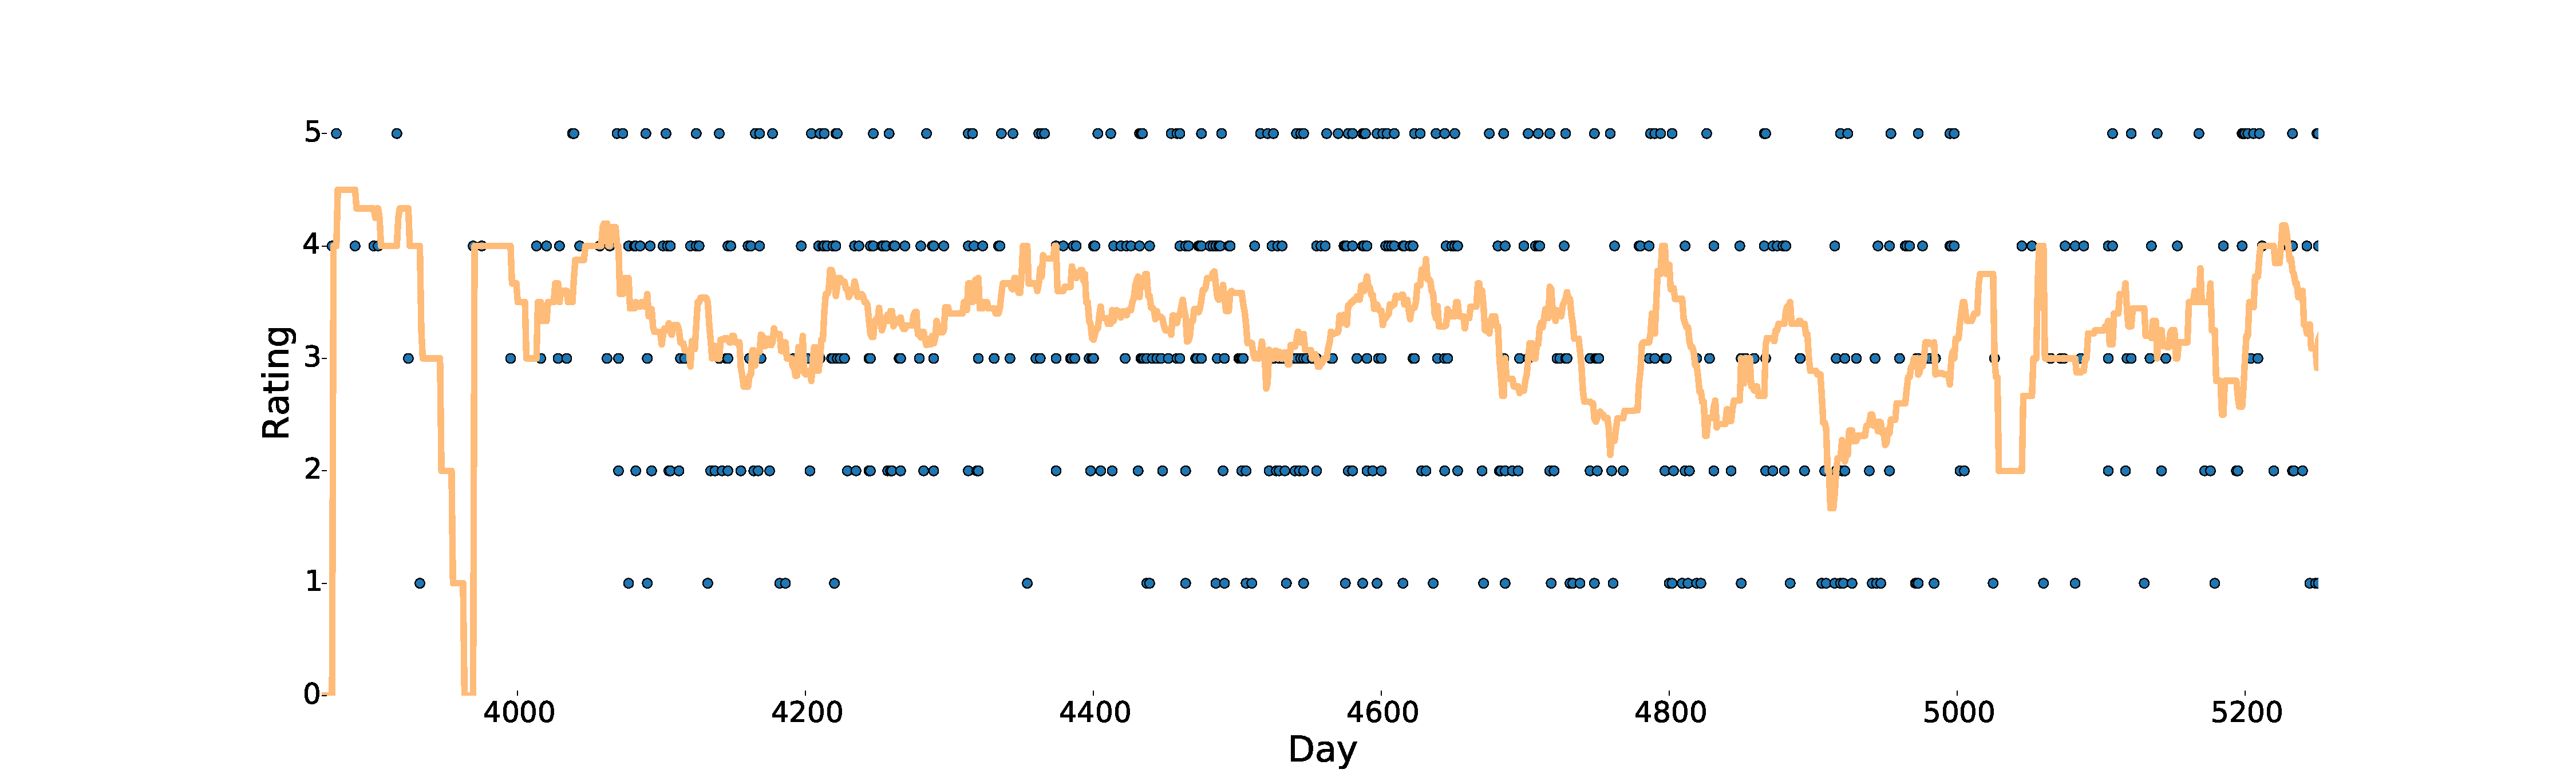
\includegraphics[width=\linewidth]{moving_avg.pdf}
\caption{ Moving average of ratings for a specific business}
\label{fig:moving_average}
\end{figure}

\subsection{Clustering}
We checked different clustering algorithms and for the same number of clusters, K-Means based on the geographic locations of businesses had the best result. The result of two clustering algorithms results are shown in Figure~\ref{fig:clusters}.  As we can see DBSCAN is not giving a good result. Since in a city there are so many businesses acting like bridges that connect two big clusters together. This is the main reason that in the business clustering problem DBSCAN is not performing as good as K-Means.

\begin{figure}[h]
\centering
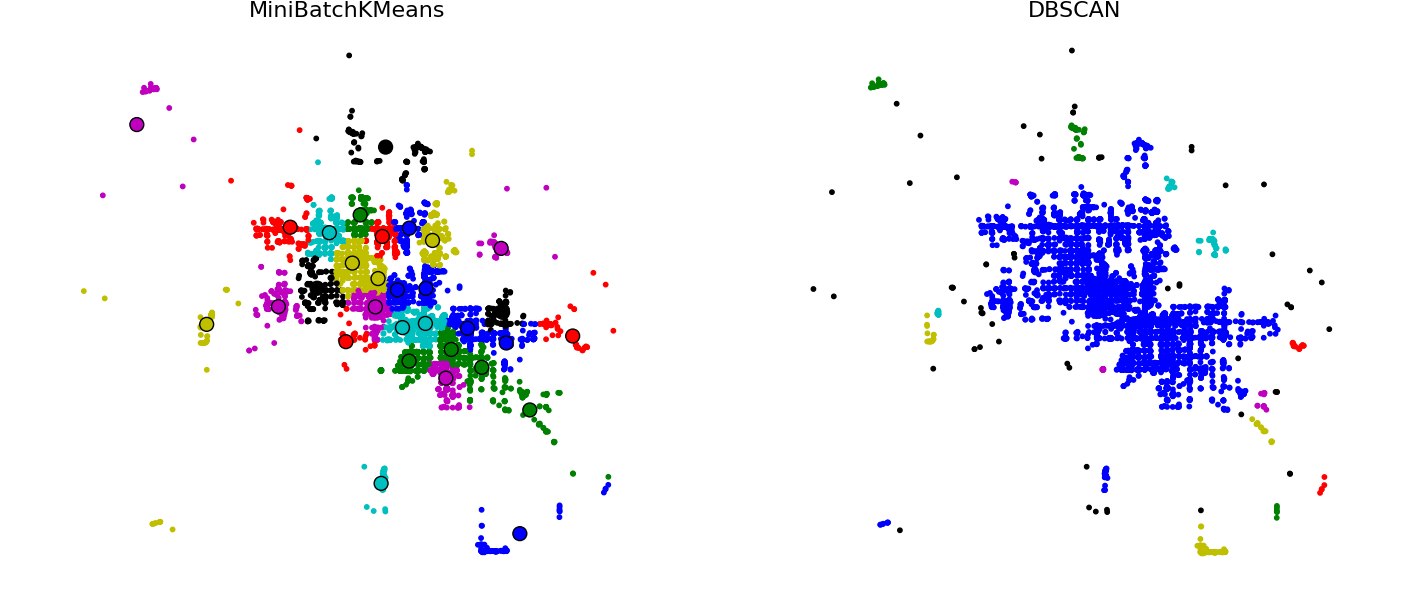
\includegraphics[width=\columnwidth]{clusters.png}
\caption{ K-Means and DBSCAN clustering}
\label{fig:clusters}
\end{figure}

As we previously described in the introduction, we are interested to look at clusters of businesses.
The first step in our project is thus to find a good way of clustering businesses.
We found that using zip codes to group businesses is ineffective as groups of businesses often span zip code boundaries.
We experimented with multiple clustering methods and ended up using k-means clustering with the geographical location as features because we are interested to observe interaction between businesses that are physically close to each other. Using k-means we are taking the advantage of clustering close businesses together and also putting far businesses that are not influencing each other into different clusters. In this case we can assume that the businesses in two different clusters are independent, and only businesses in one cluster influence each others behaviors. We will have a brief overview on the different clustering techniques used and a benchmark that reasons which one works the best in the case of our study.

\section{Features}
In various domains, like text learning, image classification, and specially cases where there are many features compared to data samples feature selection techniques are used. The feature sets selected for our model plays an important role to define a better feature similarity measure which can lead to improvement of our prediction algorithms and also finding correlations between different businesses.
Once feature which is used to find the correlations of business ratings in Section~\ref{sec:correlation_of_ratings}, is the moving average of ratings stars. This feature gives us an understanding of how a business was performing in a period of time and how the users rated that specific business in that time.

Since the motivation is predicting the impact of the businesses within a cluster, it is natural to consider pairwise metrics when constructing the features for the models. To this end, we constructed features out of the pairwise comparison of the attributes of the businesses in the dataset. Some of the business attributes in the dataset are:
\begin{itemize}
  \item Type of the business: restaurant, lounge, etc.
  \item Price Range: \$, \$\$, ...
\end{itemize}

We tried three different sets of features.

First set of features: Assign a feature vector for a pair of businesses. Every feature in the vector is either 1 or -1 and corresponds to an attribute in the dataset. Value assignment of the features is as follows:
\begin{itemize}
\item 1: the two businesses have the same (if attribute is discrete) or strongly overlapping (if the attribute is continuous) values for the corresponding attribute
\item -1: the two businesses have the different (if attribute is discrete) or non-overlapping (if the attribute is continuous) values for the corresponding attribute
\end{itemize}

Second set of features: The structure is the same as the first set of features, with the difference that each feature can have 3 values:
(sub bullets?)
\begin{itemize}
\item 2: the two businesses have the same (if attribute is discrete) or strongly overlapping (if the attribute is continuous) values for the corresponding attribute
\item 1: one of the two businesses has a given attribute but not the other
\item 0: none of the businesses have a given attribute
\end{itemize}

Third set of features: For all continuous values, we use the distance as a feature and we concatenate the binary features of the two businesses.


\section{Models}
All the analysis in the project was based on using the pairwise features outlined above for predicting pairwise metrics to be defined in what follows.
Specifically, in this section we introduce 4 different metrics which we will henceforth call "pairwise impact metrics".

Before we move onto detailing the metrics, it is important to note a one thing we have followed regardless of the metric used: relating only businesses within a reasonable distance. We have calculated all the metrics for pairs inside the same cluster since our scope is restricted to businesses that may have pairwise relationships due to their geographical closeness. This way, we hoped to eliminate the dominance of relationships with more global causes, such as a general increasing trend to prefer mediterranian food over indian food, or frozen yogurt shops over ice-cream shops. 


\subsection*{Conditional Mean Analysis}

\begin{figure}[h]
\centering
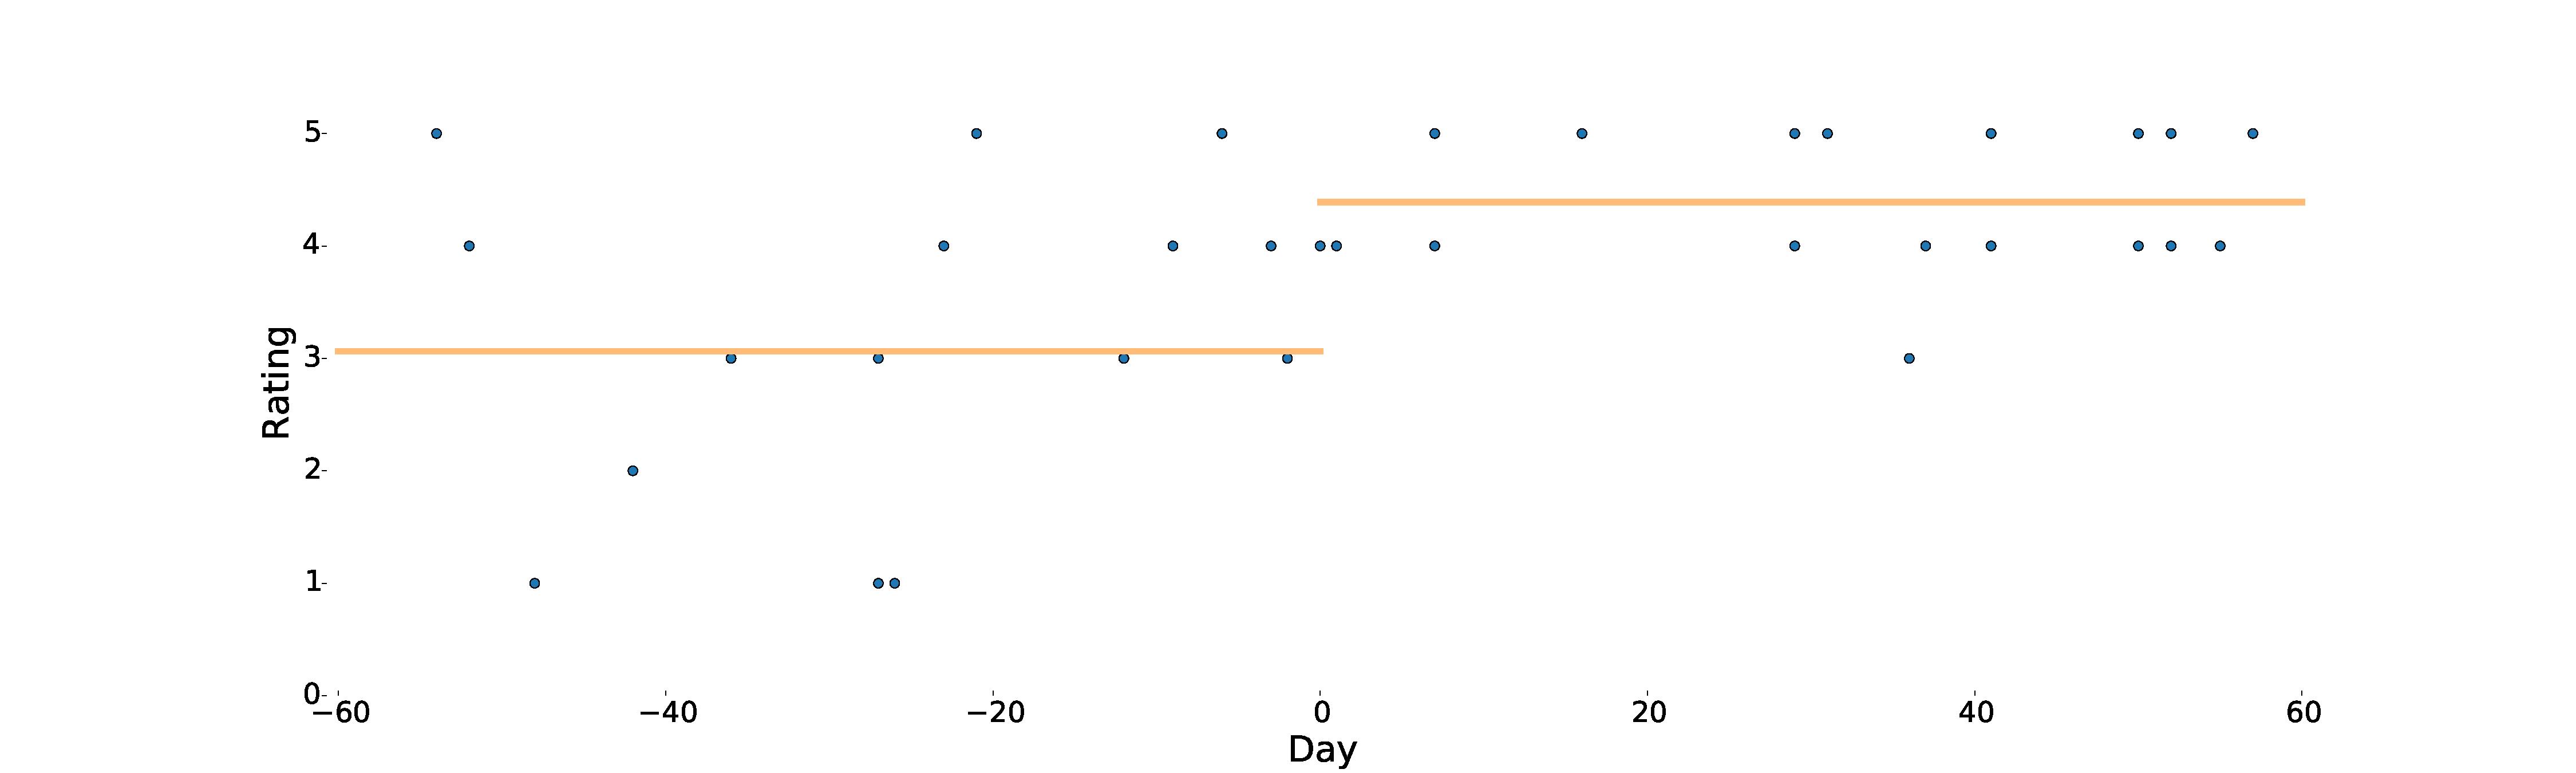
\includegraphics[width=\columnwidth]{mean.pdf}
\caption{Example mean analysis for a pair of businesses}
\end{figure}

\textbf{\textit{Hypothesis}} : Opening of a new business has an impact on the mean of ratings of the  businesses nearby.\\
\textbf{\textit{Proxy}} : Calculate the mean ratings of the nearby businesses before and after a new business opens, and get a comparative metric.\\
\textbf{\textit{Expected results}} : The change in the conditional means of the existing businesses may be predicted using the attributes of the existing businesses and the new business. \\ \\
\begin{small}
The mean ratings  were calculated as follows:\\ \\
$E_{before}(b)=\frac{1}{R_b} \sum_{x: -M+d_0\le d_x \le d_0} r_x(b),\\
E_{after}(b)=\frac{1}{R_a} \sum_{x: d_0\le d_x \le d_0+M} r_x(b)\\ \\
d_x = \small\text{day of the review x }, \\
d_0 = \small\text{opening day of the new business}, \\
r_x = \small\text{rating of review x}, \\
M = \small\text{number of days to average over}\\ $

For this analysis, we needed a date of opening for the businesses. However, we didn't have the true opening dates in the dataset, and we estimated them to be the dates of the first review for the businesses. \\
The pairwise impact metric in the conditional mean analysis was determined as $E_{before} - E_{after}$.

\label{eqn:condMean}
\end{small}



\subsection*{Trend Analysis}
\begin{figure}[h]
\centering
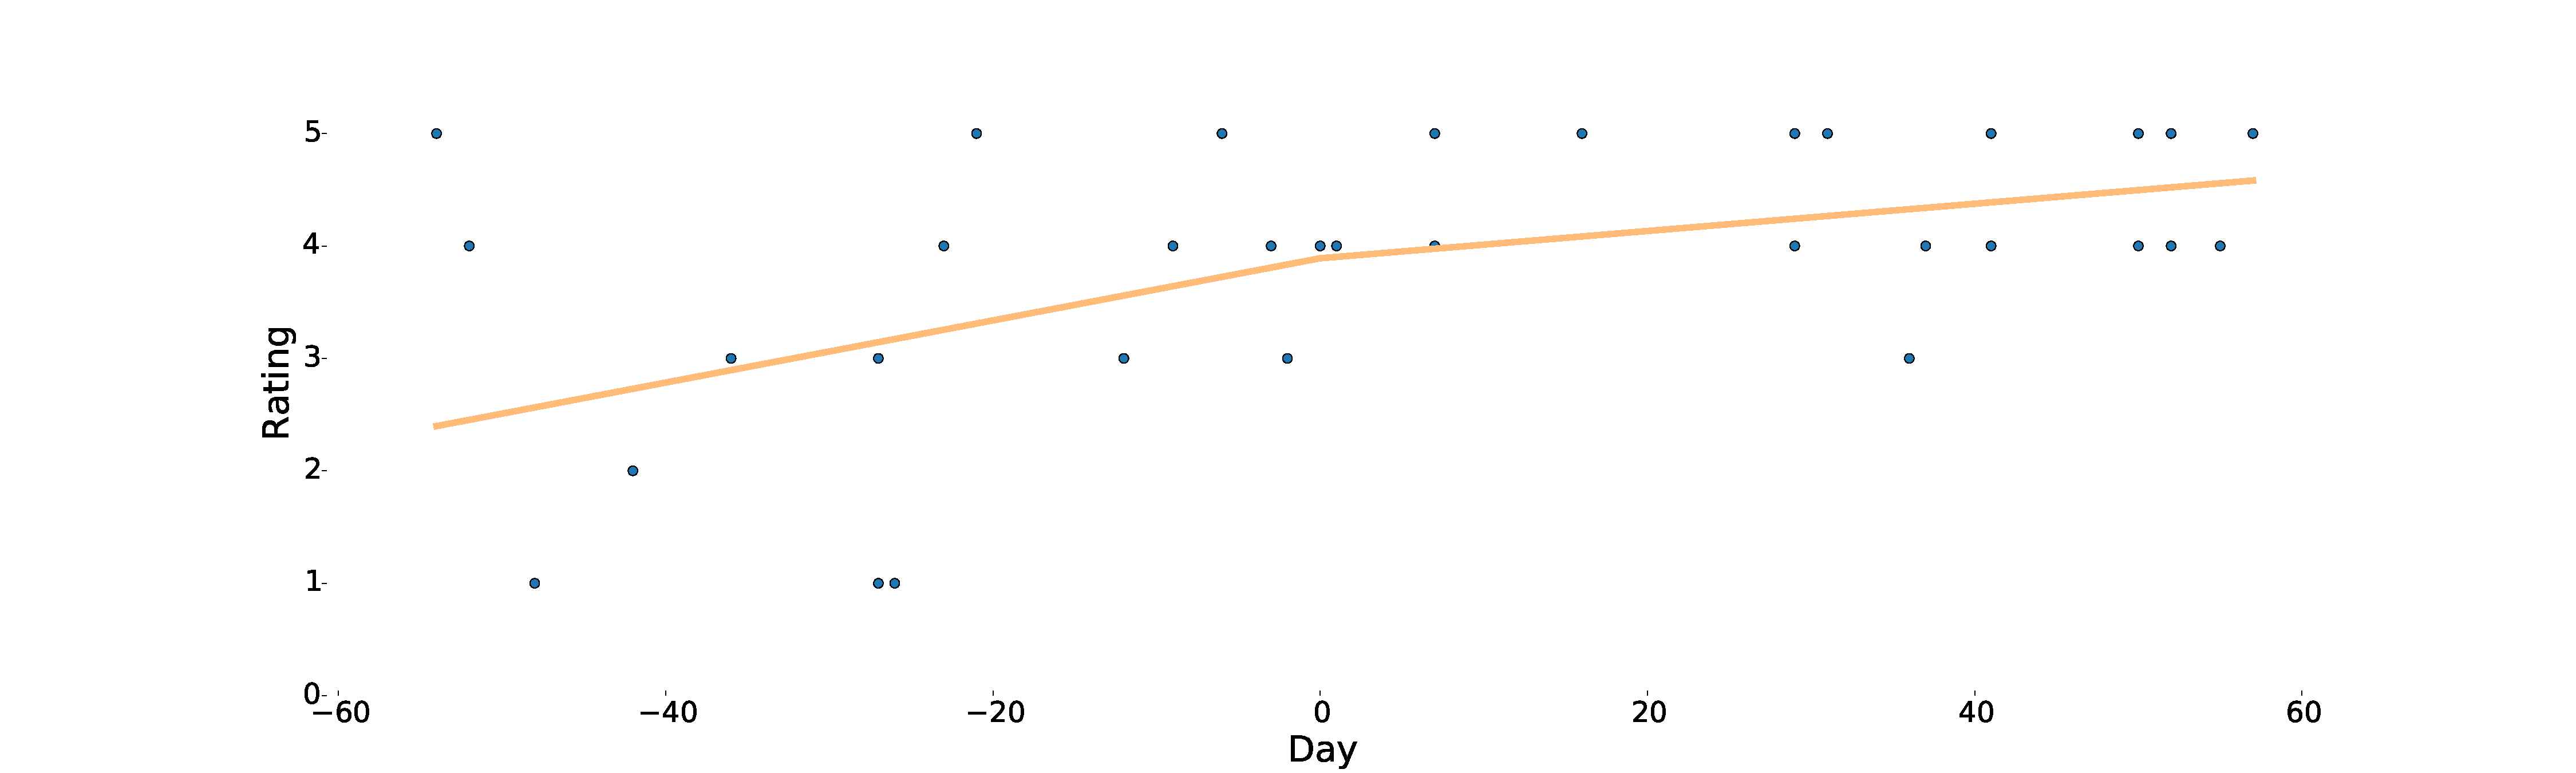
\includegraphics[width=\columnwidth]{trend.pdf}
\caption{Example trend analysis for a pair of businesses}
\end{figure}

\textbf{\textit{Hypothesis}} : Opening of a new business has an impact on the trends of ratings of the businesses nearby.\\
\textbf{\textit{Proxy}} : Fit separate lines for the ratings of a business both before and after a new business opens in the neighborhood. Calculate a metric based on the difference in the slopes of the two lines.\\
\textbf{\textit{Expected results}} : The change in the trends of the existing businesses with respect to the launching  of a new business in the neighborhood may be predicted using the attributes of the existing businesses and the new business. 

First, we estimated the opening date of the businesses as explained in the previous subsection. Then, for each pair of businesses we fit two lines for the ratings of the older business around the origin (the estimated opening date of the newer business) within a specified time window, imposing that the lines touch at the origin . Specifically, we are solving the following least squares problem:
\begin{equation*}
 \left [\begin{array}{ccc}x_{before} & 0 & 1 \\
 0 & x_{after} & 1 \end{array} \right ] 
  \left [\begin{array}{c}s_1 \\ s_2 \\ c \end{array} \right ] 
 =  \left [\begin{array}{c}y_{before} \\ y_{after} \end{array} \right ] ,
\end{equation*}
where $x_{before}$  ($x_{after}$) is a vector of the days of filtered ratings of the older business before (after) the newer business opens, $y_{before}$  ($y_{after}$) is a vector of filtered ratings of the older business before  (after) the newer business opens, $s_1$  ($s_2$) is the slope of the line fitted to the ratings of the older business before  (after) the newer business opens, and $c$ is the common intercept for the two lines. One thing to note here is that the elements of $x_{before}$ and $x_{after}$ are shifted such that the last element of $x_{before}$ is 0 and the first element of $x_{after}$ is 1.

The pairwise impact metric was determined to be the difference in the angles of the two slopes. 

\subsection*{General Trend Analysis}

\begin{figure}[h]
\centering
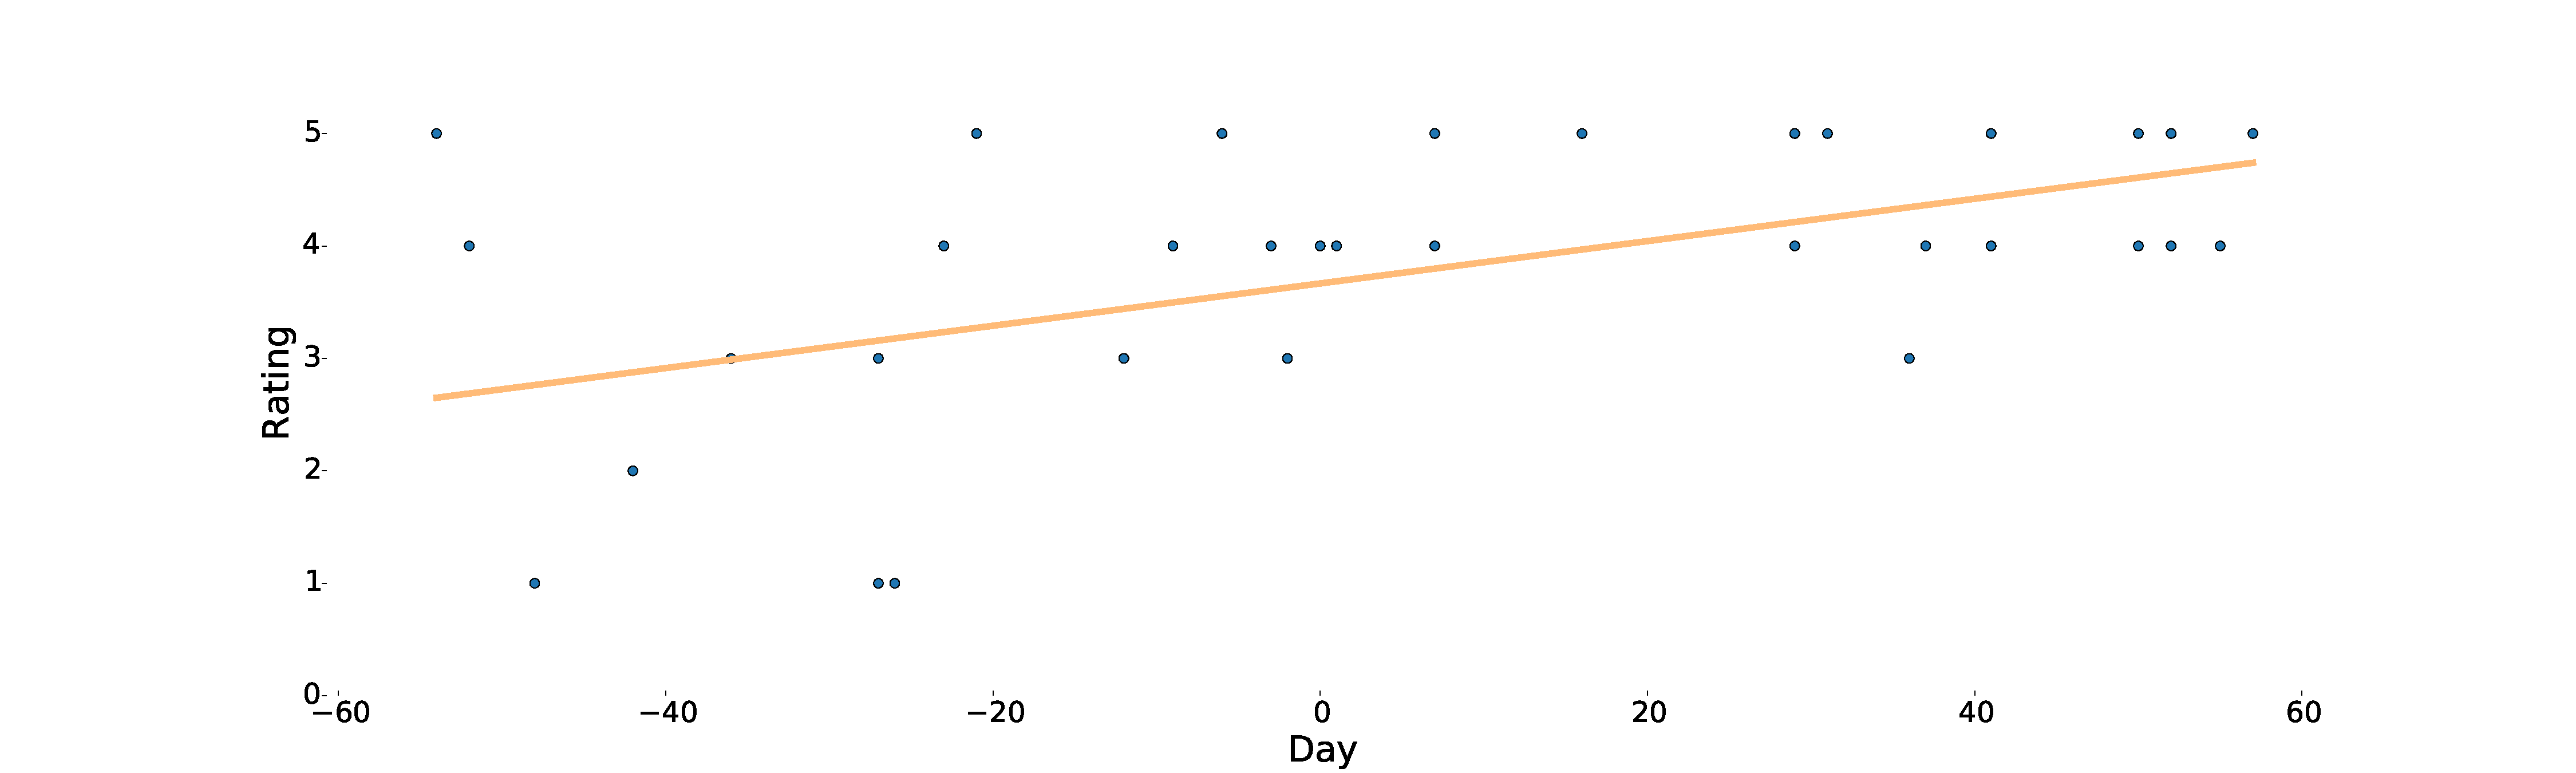
\includegraphics[width=\columnwidth]{gen_trend.pdf}
\caption{   Example general trend analysis for a pair of businesses}
\end{figure}

\textbf{\textit{Hypothesis}} : The exact opening date is not known and since prediction is noisy, the trend analysis might fail. The general trends of the existing businesses around a rough estimate of the opening time of a new business may reflect (with less noise compared to the trend analysis) the impact of the new business on them.\\
\textbf{\textit{Proxy}} : Fit a single line for the ratings of a business around the estimated opening date of a newly opened business in the neighborhood. Determine if the business has an increasing or a decreasing trend based on the slope of the line.\\
\textbf{\textit{Expected results}} : The general trends of the existing businesses around the launching date of a new business in the neighborhood may be predicted using the attributes of the existing businesses and the new business. 

The method to apply was very similar to that for the trend analysis, with the distinction being that for general trend analysis we fitted a single line for the whole time window and calculated a single slope. Mathematically, we calculated the least square solution to the following equation:
\begin{equation*}
 \left [\begin{array}{c}x_{before} \\ x_{after}  \end{array} \right ] 
  \left [\begin{array}{c}s \\ c \end{array} \right ] 
 =  \left [\begin{array}{c}y_{before} \\ y_{after} \end{array} \right ] ,
\end{equation*}
with everything except for $s$ is as defined in the previous subsection. $s$ is the slope to the fitted line for the whole time window .

The pairwise impact metric in general trend analysis was determined to be the slope of the fitted line($s$). 

\begin{table*}[ht!]
\centering
\begin{tabular}{@{}llrrrr@{}}
\toprule
                                                              &                     & \multicolumn{2}{c}{sig/insig classif.} & \multicolumn{2}{c}{pos/neg classif.} \\ 
\cmidrule(r){3-4}
\cmidrule(r){5-6}
                                                              &                     & \multicolumn{1}{c}{60 days} & \multicolumn{1}{c}{90 days} & \multicolumn{1}{c}{60 days} & \multicolumn{1}{c}{90 days} \\ \midrule
\multirow{2}{*}{Conditional Mean}  & SVM rbf             &   0.84/0.61   &  0.82/0.60  & 0.84/0.60 &  0.85/0.65  \\
                                        & Logistic Regression & 0.61/0.52  & 0.60/0.52 &  0.56/0.49   &  0.56/0.49   \\ \midrule
\multirow{2}{*}{Trend Analysis}       & SVM rbf             & 0.83/0.62    &  0.82/0.59 & 0.84/0.60 & 0.81/0.58   \\
                                        & Logistic Regression &  0.60/0.55   & 0.58/0.48 &  0.57/0.49  &  0.56/0.51   \\ \midrule
\multirow{2}{*}{General Trend Analysis} & SVM rbf             & 0.84/0.62 & 0.80/0.62 &  0.81/0.60 &  0.83/0.63  \\
                                       & Logistic Regression &  0.59/0.52  & 0.58/0.54  &   0.57/0.49  &   0.58/0.49       \\ \midrule
\multirow{2}{*}{Correlation Analysis}   & SVM rbf             & \multicolumn{2}{c}{0.85/0.81}  & \multicolumn{2}{c}{0.86/0.81} \\
                                        & Logistic Regression & \multicolumn{2}{c}{0.84/0.82}  & \multicolumn{2}{c}{0.86/0.83} \\
\bottomrule
\end{tabular}
\caption{Training and 10-fold cross-validation score for predictions}
\label{tab:results}
\end{table*}

\subsection*{Correlation Analysis}
The correlation coefficient is a measure of linear association between two variables. A high positive correlation indicates that two variables are perfectly related in a positive linear sense, and a high negative correlation indicates that two variables are perfectly related in a negative linear sense. And zero means that they are not related at all. This show that studying the business correlation give us a very good intuition on how businesses are effecting each other. 

\begin{figure}[h]
\centering
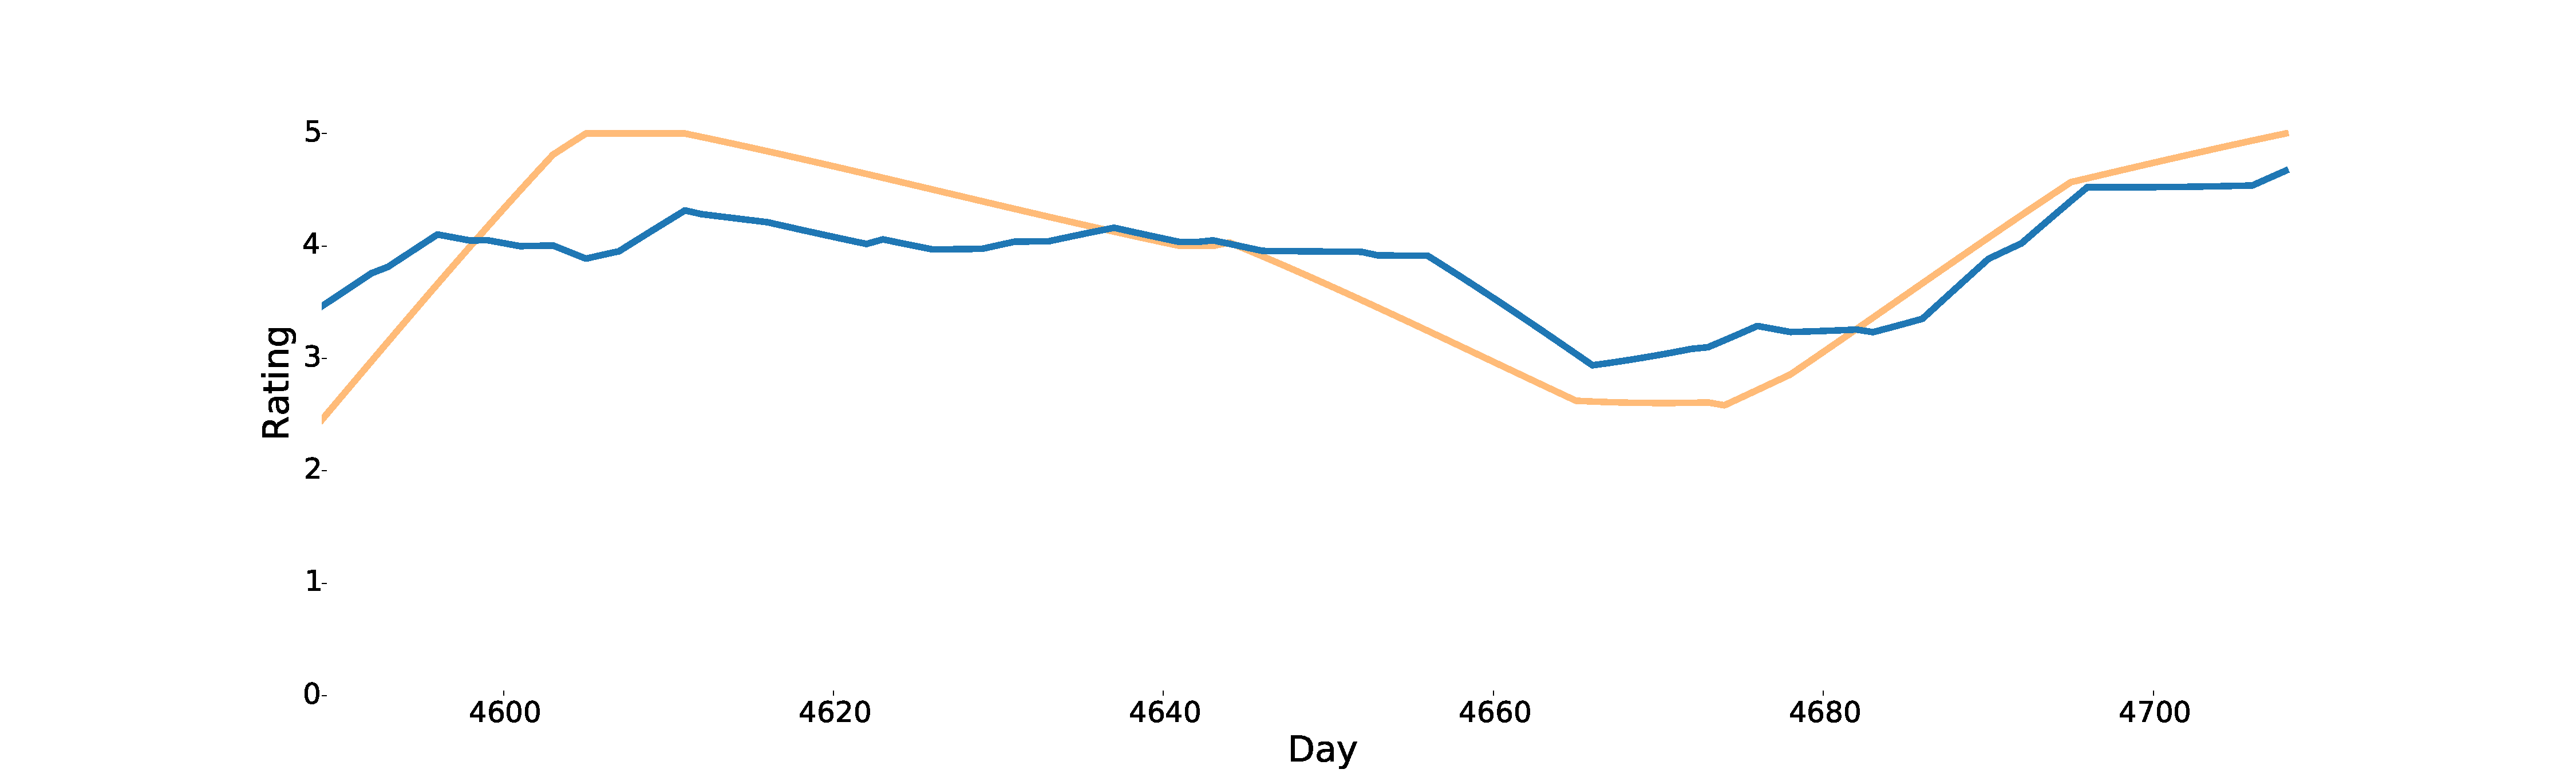
\includegraphics[width=\columnwidth]{corr.pdf}
\caption{Example of correlation analysis for a pair of businesses}
\end{figure}

\textbf{\textit{Hypothesis}} :The correlation between the  time-series of average star ratings between businesses may serve as a low noise (as compared to metrics discussed above) metric as it reflects a pairwise relationship over a long period of time.\\
\textbf{\textit{Proxy}} : Compute the correlation of ratings over time.\\
\textbf{\textit{Expected results}} : The correlation can be predicted using the attributes of the businesses within reasonable distance. 

\begin{figure}
\centering
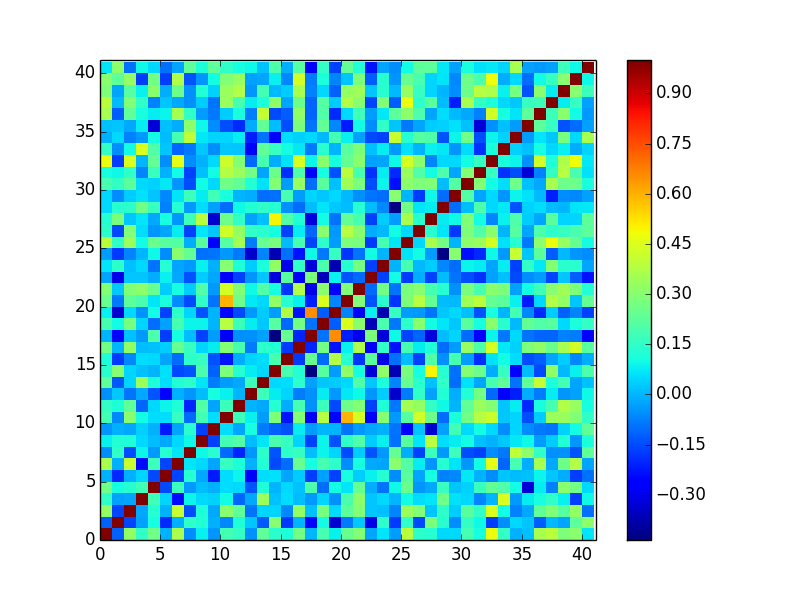
\includegraphics[width=\columnwidth]{cov_cluster_28}
\caption{Correlation between ratings of 41 businesses in an example cluster}
\label{fig:covmat}
\end{figure}
After choosing one cluster, we analyzed the correlation of ratings between different businesses inside the cluster.
To do so, we first applied a Gaussian filter to the time series of ratings to smooth out local fluctuations in ratings. The correlation coefficient between the ratings were then calculated as:

\begin{align*}
    \rho_{XY} &= \frac{E(XY)}{\sqrt{E(X^2) E(Y^2)}} \\
    E(X) &= \frac{1}{n} \sum_{t = 0}^{n} r_t
\end{align*}

Where $r_t$ is the filtered rating.
In this step we discarded all businesses with a low number of ratings because they potentially would not provide not enough signal to get a good estimate for the correlation.

As Figure~\ref{fig:correlation} shows, there are a quite a few cases with strong correlation.

The pairwise impact metric was determined to be the correlation coefficient. 
%----------------------------------------------------------------------------------------
%	RESULTS 
%----------------------------------------------------------------------------------------

\section{Results}
%
There were so many tools we used for getting the results. The main tools for our study was Python to preprocess and analyze the data and the Scikit package \cite{pedregosa2011scikit} to perform the machine learning tasks.
We found that the previously presented two sets of features performed very similarly.
This indicates that the difference in attributes gives us enough information for the predictions that we studied.
Thus, we are only presenting the results for the first feature set.


We did two types of experiments: (a) classification of positive vs. negative values for all the metrics and (b) classification of significant vs. insignificant values (absolute value bigger than a certain threshold) for all models. Converting the metrics to binary features was exacly the same for all the metrics due to their conceptual correspondance. We also adjusted the thresholds to have an even distribution of the class labels in order to avoid bias in the classification accuracy.

For every model except correlation analysis, we also considered different lengths of periods to fit the model.
We found that there were only minor differences between a period of 60 days and 90 days.

Table~\ref{tab:results} contains the mean training score and the 10-fold cross-validation score for predictions in a single cluster.
We used support vector classifier(SVM) with gaussian kernel and logistic regression with l1-norm regularization for all the tests.
The cluster consists of 147 businesses which corresponds to 10730 pairings.

We also collected results for linear, polynomial and sigmoid kernels for SVM classifier but we omitted them here due to their poor performance.

\section{Discussion}

Out of the 4 different pairwise impact metrics that we have made effort to predict, we were most successful with the correlation metric ($>80\%$ CV accuracy with both classifiers for both classification experiments). 
One thing that we have noted is that SVM performed significantly superior to logistic regression for the conditional mean analysis, trend analysis, and general trend analysis, whereas it was outperformed slightly in the correlation analysis. We have speculated that this might be due to possible effective "noise" level from the first 3 metrics being significantly higher than that from the correlation metric. 
SVM is able to fit better with the presence of noise due to its possibly higher VC dimension compared to that of logistic regression with l1 regularization.(Overfitting behavior of SVM compared to logistic regression classifier is also evident in the first 3 rows of Table~\ref{tab:results}). 
However, given higher "signal to noise" ratio (hence cleaner data), which we believe is present in the correlation metric, it loses its comparative advantage against logistic regression. 

Following up from this idea, we have gone back to the calculating the first three metrics and chose different values for the opening dates for the new businesses around the previously estimated values. In quite a few cases, we have observed considerable changes in the values for the metrics (data not shown, however on average 15-20\% of the pairwise metric values in the cluster of interest have shown considerable variation, with the majority of the pairwise values effected at different levels). This observation supports our suspicions about the discrepancies in the classification accuracies.

One last thing worth mentioning is that, for the correlation analysis, the training accuracies were quite close to the 10 fold CV accuracies ($\le 3\%$ difference for logistic regression and $\le 5\%$ difference for SVM, last row of Table~\ref{tab:results}). This fact suggests that the relationships between businesses within cluster are predicted accross disjoint subpopulations inside the cluster. This is important in answering the practical question of whether the correlation between any two novel businesses may be predicted by using a precalculated predicted model.

\section{Conclusion}
We tried to predict the interaction of two businesses with multiple models.
The quality of our predictions turned out to be relatively low for most models.
Possible reasons are:
\begin{itemize}
\item The rating data is noisy and sparse at the same time. Most businesses don't have ratings every day and the variance of the ratings for a given time period is high.
\item The training score of SVM is high in general but the cross-validation score is low in a lot of cases which may be a hint that SVM is overfitting.
\item For the conditional mean analysis and the trend analysis, we assume that the opening date of the business is close to the first review submitted for the business. This might not always be the case.
\end{itemize}

We achieved good results when predicting correlation and this shows that our approach has merit.
We also observed that SVM generally outperformed logistic regression in cases other than correlation analysis.

\section{Future Work}
We have already performed different types of clustering on the data and chose the best one based on the geographical location of the businesses. It would be interesting to perform other types of clustering techniques based on the features distance metrics described in the features section, and study how the correlated businesses are geographicly located. This would allow us to analyze the structure of a cluster, e.g. whether a given cluster consists of many similar businesses (for example Chinatown in San Francisco) or whether a cluster is heterogenous (for example the Great Mall).\\
Since we have used very common business attributes like geographic distance, open hours, business types, and similar common features for our studies, we have the advantage to do the same experiments on similar datasets. In the future, it would be interesting to see if similar or even better observations can be made on different datasets, where more information on the businesses is available. In addition it would be interesting to look interactions between businesses other than the opening of a new business.

% The following two commands are all you need in the
% initial runs of your .tex file to
% produce the bibliography for the citations in your paper.
\bibliographystyle{abbrv}
\bibliography{references}  % vldb_sample.bib is the name of the Bibliography in this case

\end{document}
